% Created 2023-02-28 Tue 20:18
% Intended LaTeX compiler: lualatex
\documentclass[bigger]{beamer}
\usepackage{graphicx}
\usepackage{longtable}
\usepackage{wrapfig}
\usepackage{rotating}
\usepackage[normalem]{ulem}
\usepackage{amsmath}
\usepackage{amssymb}
\usepackage{capt-of}
\usepackage{hyperref}
\usetheme[progressbar=foot, sectionpage=none, numbering=fraction]{metropolis}
\usepackage{tikz}
\usepackage{booktabs}
\usepackage{adjustbox}
\usepackage{diagbox}
\usepackage{latexcolors}
\usetikzlibrary{automata, positioning, arrows, arrows.meta}
\usepackage{diagbox}
\usepackage{dsfont}
\usepackage{amsmath}
\usepackage{fontawesome5}
\definecolor{RedBrown}{RGB}{192, 4, 4} \setbeamercolor{progress bar}{fg=RedBrown} \setbeamercolor{title separator}{fg=RedBrown}
\setbeamercolor{progress bar in head/foot}{fg=RedBrown} \setbeamercolor{progress bar in section page}{fg=RedBrown} \setbeamercolor{alerted text}{fg=RedBrown}
\pretocmd{\tableofcontents}{\thispagestyle{empty}}{}{}
\addtocounter{framenumber}{-1}
\usepackage{listings}
\usepackage{xcolor}
\definecolor{codegreen}{rgb}{0,0.6,0}
\definecolor{codegray}{rgb}{0.5,0.5,0.5}
\definecolor{codepurple}{rgb}{0.58,0,0.82}
\definecolor{backcolour}{HTML}{f0f0f0}
\lstdefinestyle{mystyle}{
backgroundcolor=\color{backcolour},
commentstyle=\color{codegreen},
keywordstyle=\color{magenta},
numberstyle=\tiny\color{codegray},
stringstyle=\color{codepurple},
basicstyle=\ttfamily,
breakatwhitespace=false,
breaklines=true,
captionpos=b,
keepspaces=true,
numbers=none,
numbersep=5pt,
showspaces=false,
showstringspaces=false,
showtabs=false,
tabsize=2
}
\lstset{style=mystyle}
\usetheme{default}
\author{Andrea Pierré}
\date{February 27\textsuperscript{th}, 2023}
\title{Joint RL meeting}
\subtitle{Gridworld implementation of Olivia's task (bis)}
\institute{Brown University}
\titlegraphic{\hfill
\includegraphics[height=1.5cm]{img/Brown Logo_2016_2 Color Process ST_1300.png}}
\setbeamercovered{transparent=10}
\setbeamertemplate{section in toc}[sections numbered]
\AtBeginSection[]{\begin{frame}[plain, noframenumbering]{Outline}    \setbeamertemplate{section in toc}[sections numbered]\setbeamertemplate{subsection in toc}[subsections numbered]\tableofcontents[currentsection, currentsubsection]\end{frame}}
\AtBeginSubsection[]{\begin{frame}[plain, noframenumbering]{Outline}\setbeamertemplate{section in toc}[sections numbered]\setbeamertemplate{subsection in toc}[subsections numbered]\tableofcontents[currentsection,currentsubsection]\end{frame}}
\begin{document}

\maketitle
\begin{frame}[plain]{Outline}
\tableofcontents
\end{frame}

\section{Implementation}
\label{sec:orgc93ba6d}
\begin{frame}[label={sec:org3f2099d}]{Composite state space}
\small
\begin{itemize}
\item Allocentric setting:
\end{itemize}
\begin{center}
\begin{tabular}{ll}
\hline
location & cue\\
\hline
\{0,\ldots{},24\} & North light\\
 & South light\\
 & Odor A\\
 & Odor B\\
\hline
\end{tabular}
\end{center}
\pause
\begin{itemize}
\item Egocentric setting:
\end{itemize}
\begin{center}
\begin{tabular}{lrl}
\hline
location & head direction [°] & cue\\
\hline
\{0,\ldots{},24\} & 0 & North light\\
 & 90 & South light\\
 & 180 & Odor A\\
 & 270 & Odor B\\
\hline
\end{tabular}
\end{center}
\end{frame}
\begin{frame}[label={sec:org46c4bbf}]{Flattened state space -- allocentric setting}
\begin{columns}
\begin{column}{0.45\columnwidth}
\begin{center}
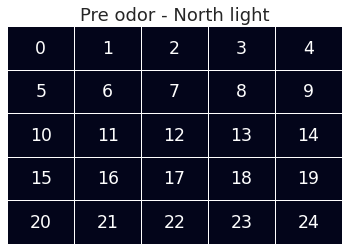
\includegraphics[width=.9\linewidth]{img/state_space_1.png}
\end{center}
\begin{center}
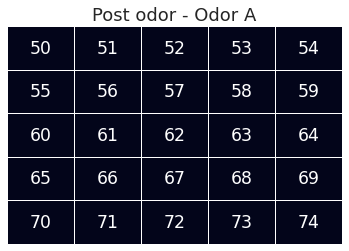
\includegraphics[width=.9\linewidth]{img/state_space_3.png}
\end{center}
\end{column}
\begin{column}{0.45\columnwidth}
\begin{center}
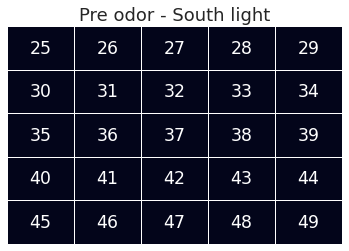
\includegraphics[width=.9\linewidth]{img/state_space_2.png}
\end{center}
\begin{center}
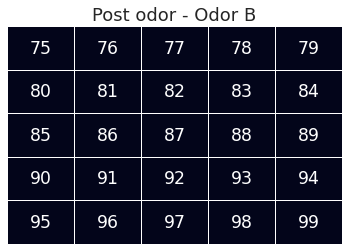
\includegraphics[width=.9\linewidth]{img/state_space_4.png}
\end{center}
\end{column}
\end{columns}
\end{frame}
\begin{frame}[label={sec:orgcc8bd0b}]{Flattened state space -- egocentric setting}
\begin{center}
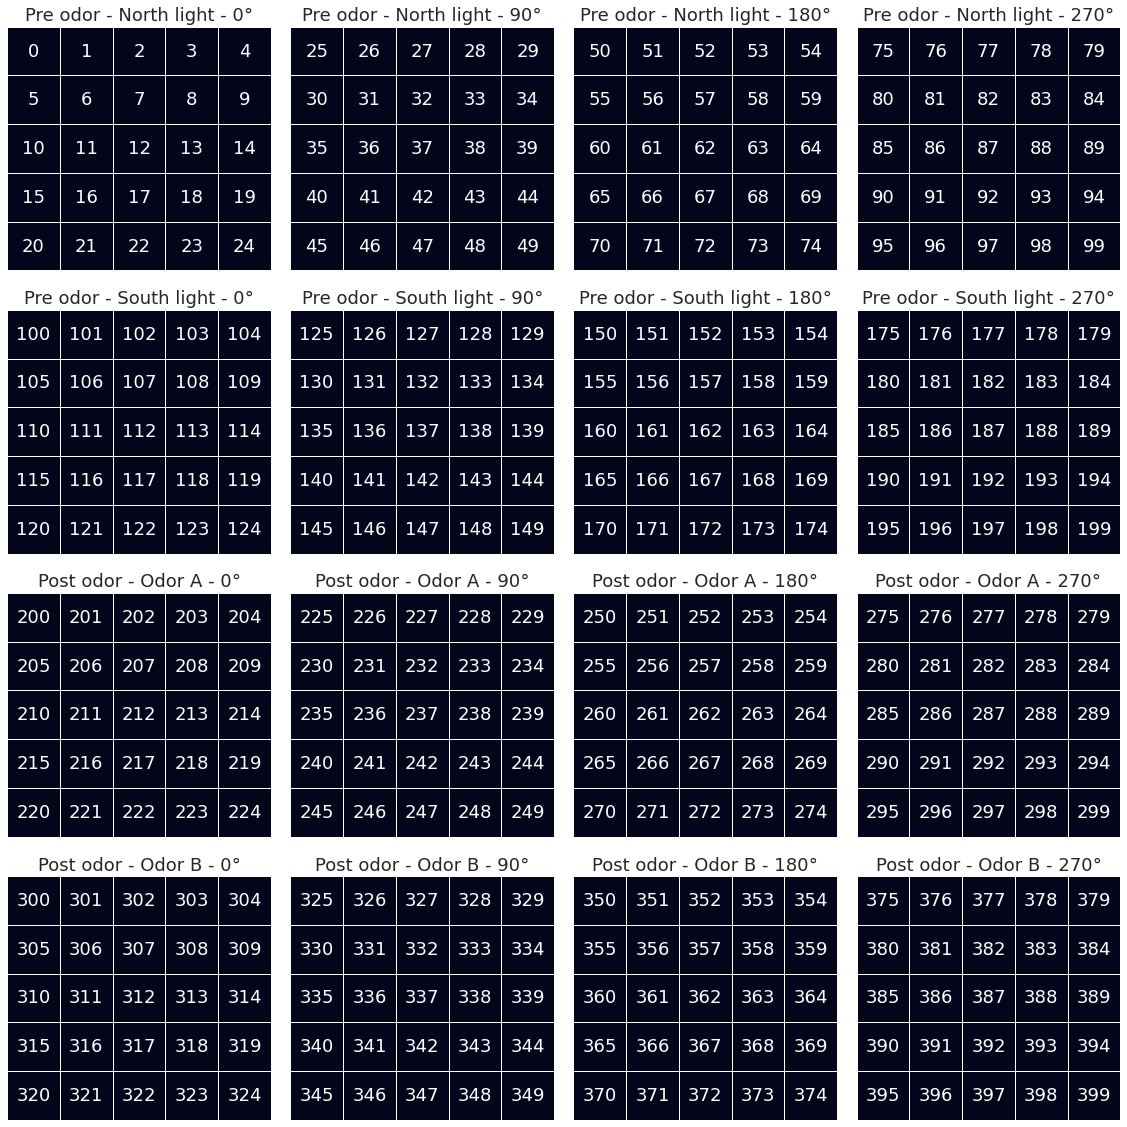
\includegraphics[height=0.9\textheight]{img/state_space_ego.png}
\end{center}
\end{frame}
\begin{frame}[<+->][label={sec:orgd2ea278},fragile]{States \& actions translation}
\begin{itemize}
\item Wrapper environment to translate the human readable environment (\alert{composite states}) into a suitable environment for the Q-learning algorithm (\alert{flat states})
\scriptsize
\begin{lstlisting}[language={Python}]
state = {"location": 13, "cue": LightCues.South}
env.convert_composite_to_flat_state(state)
# => 38
\end{lstlisting}
\begin{lstlisting}[language={Python}]
state = 63
env.convert_flat_state_to_composite(state)
# => {"location": 13, "cue": <OdorID.A: 1>}
\end{lstlisting}
\item Machine \& human friendly actions
\scriptsize
\begin{lstlisting}[language={Python}]
action = 0
Actions(action).name
# => "UP"
\end{lstlisting}
\end{itemize}
\end{frame}
\begin{frame}[label={sec:orgeaf692f}]{Algorithm troubleshooting}
Subtle bug using \(\epsilon\)-greedy when Q-values are identical:
\\[2em]
\begin{columns}
\begin{column}{0.5\columnwidth}
\centering
Vanilla \epsilon-greedy\\[2em]
\begin{center}
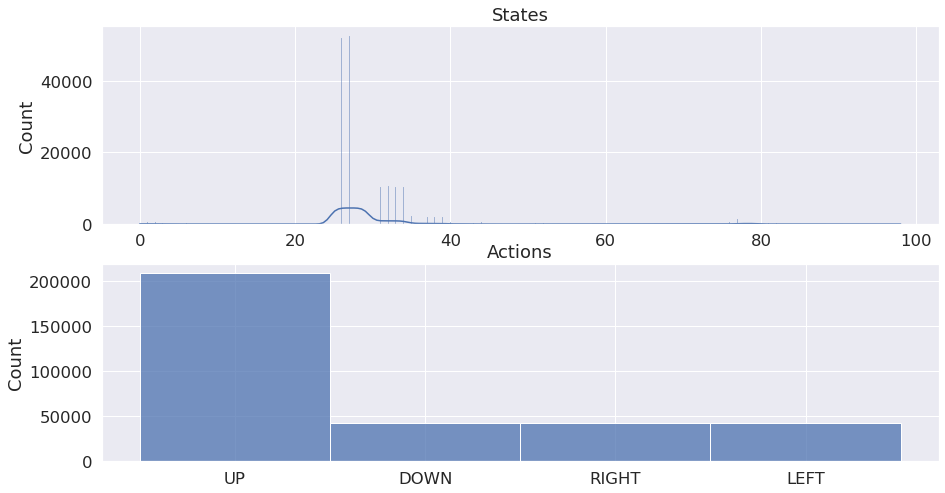
\includegraphics[width=\textwidth]{img/hist_before.png}
\end{center}
\end{column}
\begin{column}{0.5\columnwidth}
\centering
Randomly choosing between actions with the same Q-values
\begin{center}
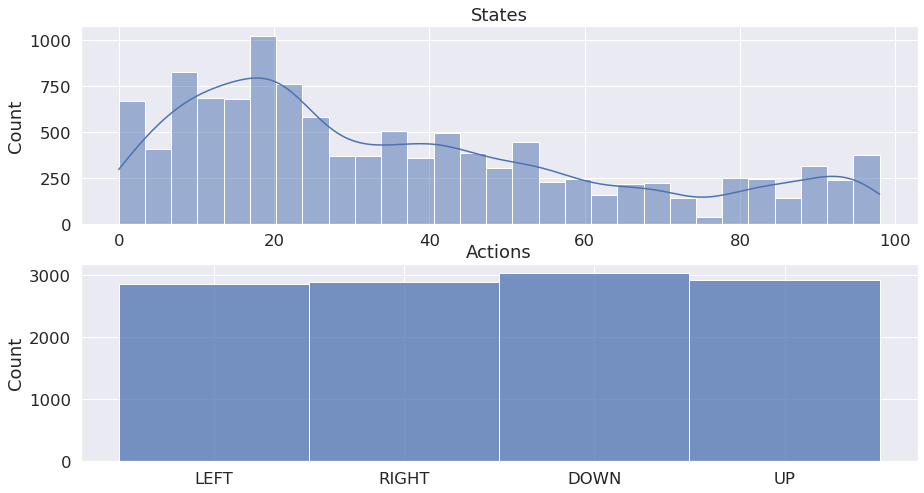
\includegraphics[width=\textwidth]{img/hist_after.png}
\end{center}
\end{column}
\end{columns}
\end{frame}
\section{Results \& experiments}
\label{sec:org2801ddb}
\begin{frame}[label={sec:org15ddb8b}]{Standard Q-learning -- allocentric setting}
\begin{center}
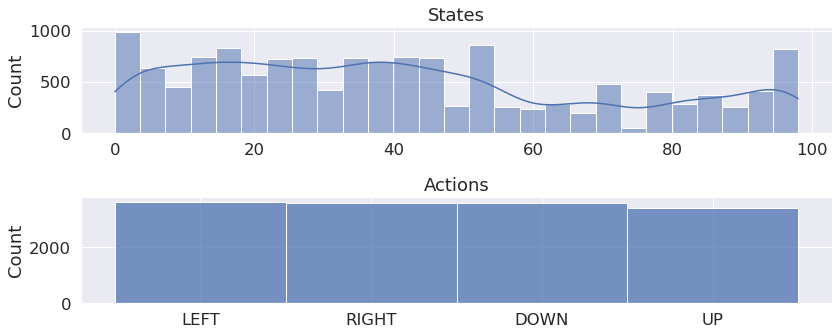
\includegraphics[height=0.4\textheight]{img/q-learning_allo_hist.png}
\end{center}
\begin{center}
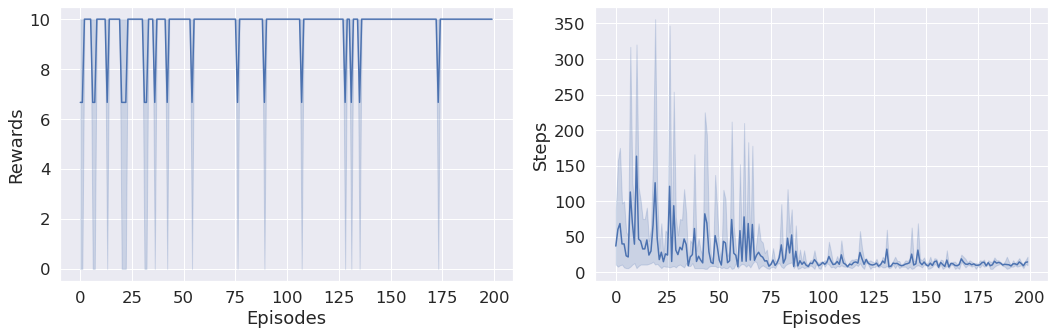
\includegraphics[height=0.4\textheight]{img/q-learning_allo_steps_rewards.png}
\end{center}
\end{frame}
\begin{frame}[label={sec:org45203f9}]{Standard Q-learning -- allocentric setting}
\begin{center}
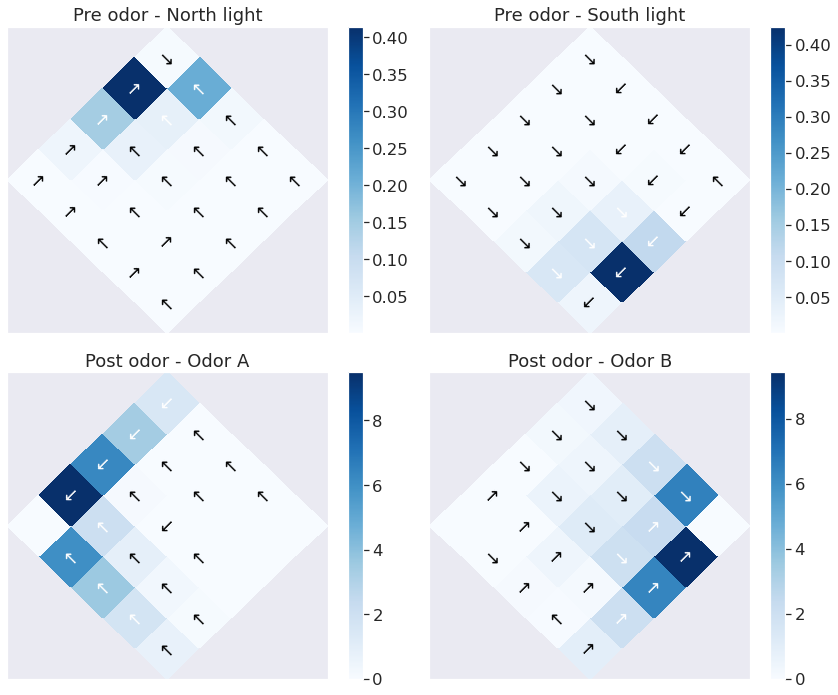
\includegraphics[width=.9\linewidth]{img/q-learning_allo_best_actions_maps.png}
\end{center}
\end{frame}
\begin{frame}[label={sec:orgd275405}]{Q-learning with function approximation -- allocentric setting -- without joint representation}
\begin{columns}
\begin{column}{0.5\columnwidth}
\begin{center}
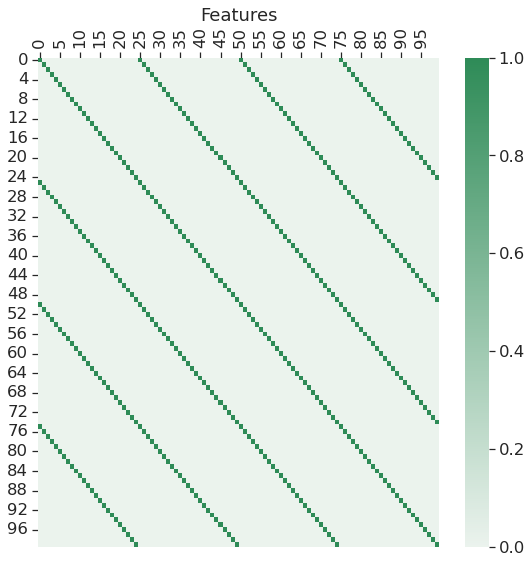
\includegraphics[height=0.4\textheight]{img/func_approx_allo_features_heatmap_nojointrep.png}
\end{center}
\end{column}
\begin{column}{0.5\columnwidth}
\begin{center}
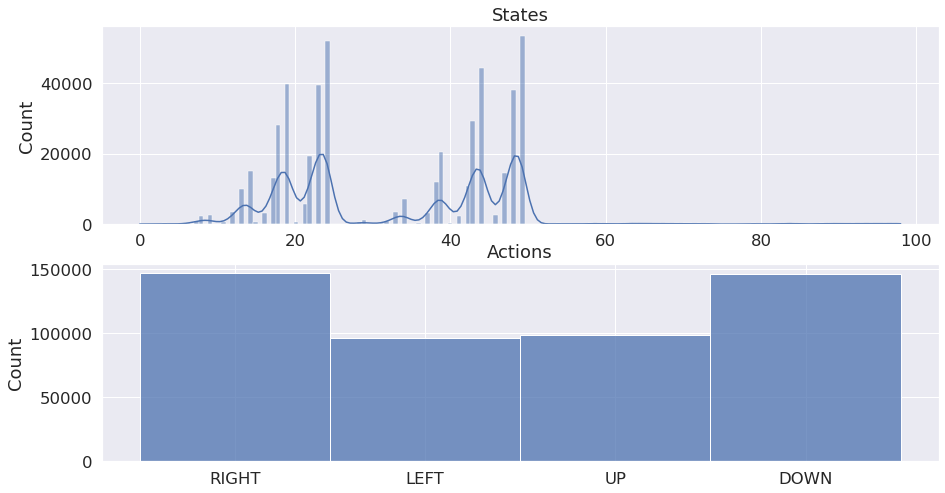
\includegraphics[width=\textwidth]{img/func_approx_allo_actions_states_hist_nojointrep.png}
\end{center}
\end{column}
\end{columns}
\begin{block}{~}
\vspace{-2em}
\begin{center}
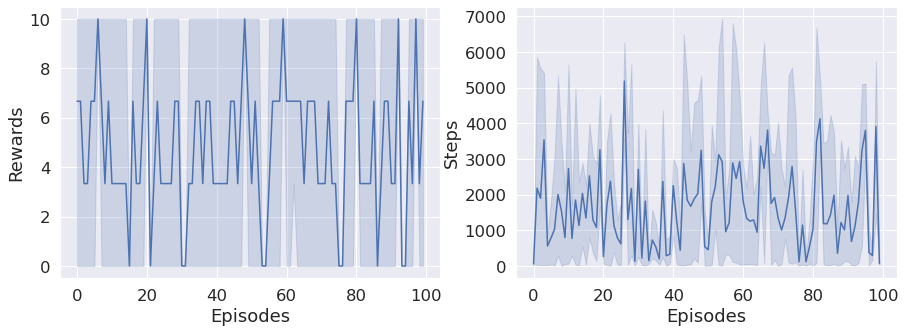
\includegraphics[height=0.4\textheight]{img/func_approx_allo_steps_rewards_nojointrep.png}
\end{center}
\end{block}
\end{frame}
\begin{frame}[label={sec:orge388911}]{Q-learning with function approximation -- allocentric setting -- without joint representation}
\begin{center}
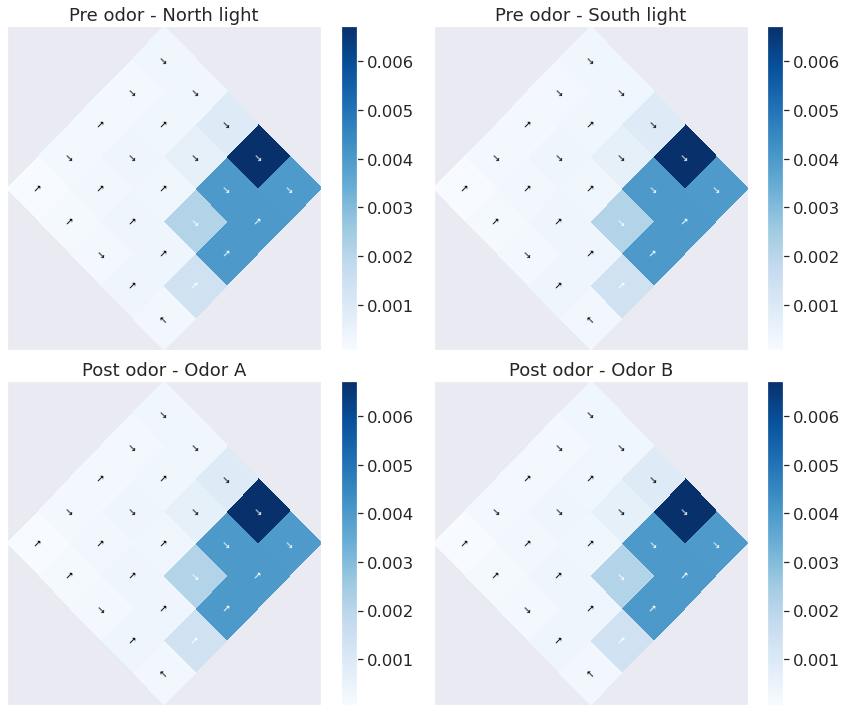
\includegraphics[height=0.8\textheight]{img/func_approx_allo_best_actions_maps_nojointrep.png}
\end{center}
\end{frame}
\begin{frame}[label={sec:org02b6431}]{Q-learning with function approximation -- allocentric setting -- with joint representation}
\begin{columns}
\begin{column}{0.5\columnwidth}
\begin{center}
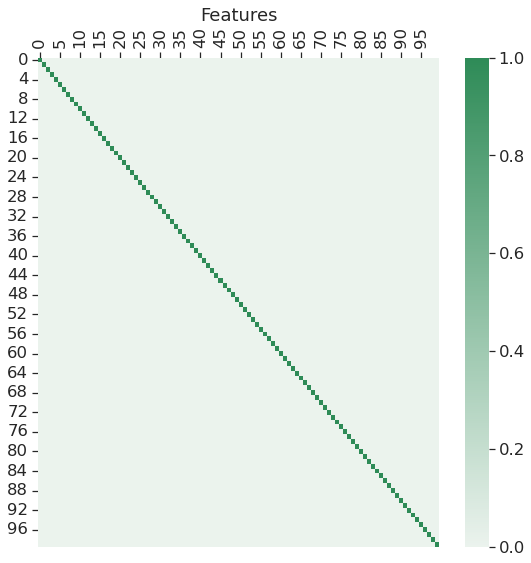
\includegraphics[height=0.4\textheight]{img/func_approx_allo_features_heatmap_jointrep.png}
\end{center}
\end{column}
\begin{column}{0.5\columnwidth}
\begin{center}
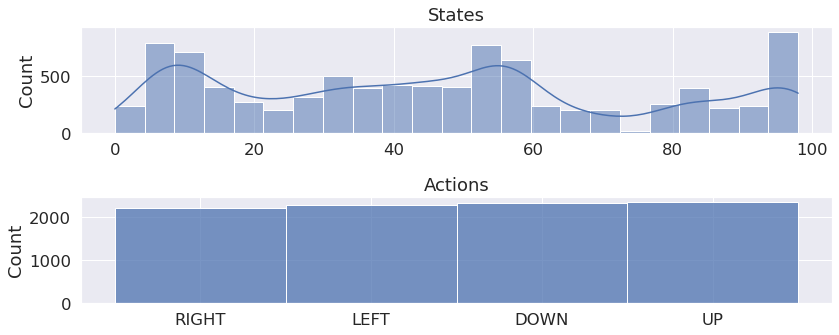
\includegraphics[width=\textwidth]{img/func_approx_allo_actions_states_hist_jointrep.png}
\end{center}
\end{column}
\end{columns}
\begin{block}{~}
\vspace{-2em}
\begin{center}
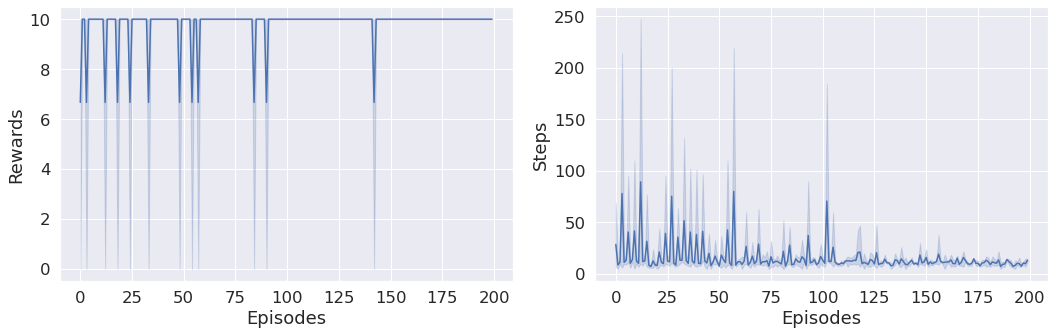
\includegraphics[height=0.4\textheight]{img/func_approx_allo_steps_rewards_jointrep.png}
\end{center}
\end{block}
\end{frame}
\begin{frame}[label={sec:orga136f2d}]{Q-learning with function approximation -- allocentric setting -- with joint representation}
\begin{center}
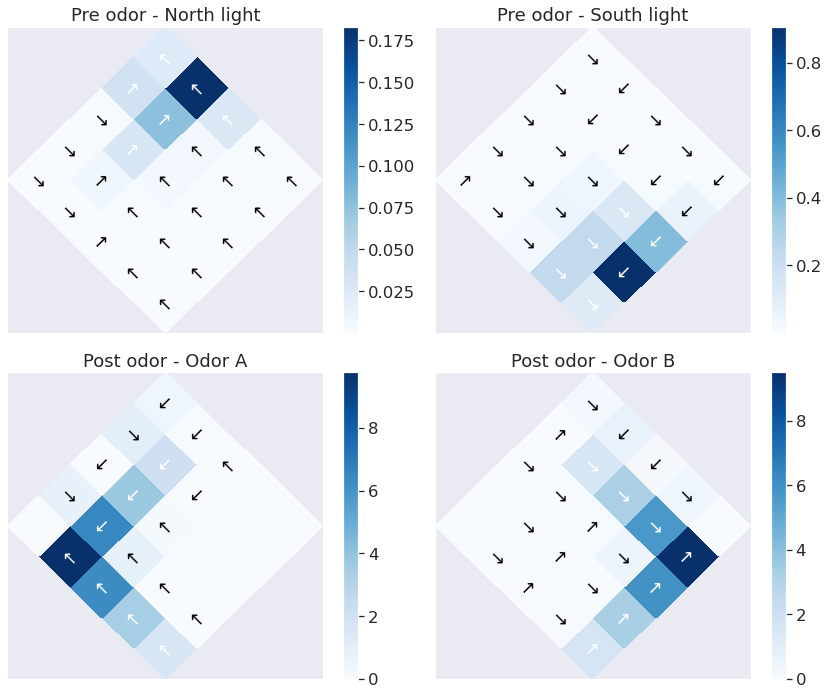
\includegraphics[height=0.8\textheight]{img/func_approx_allo_best_actions_maps_jointrep.png}
\end{center}
\end{frame}

\begin{frame}[label={sec:orgb44444a}]{Standard Q-learning -- egocentric setting}
\begin{center}
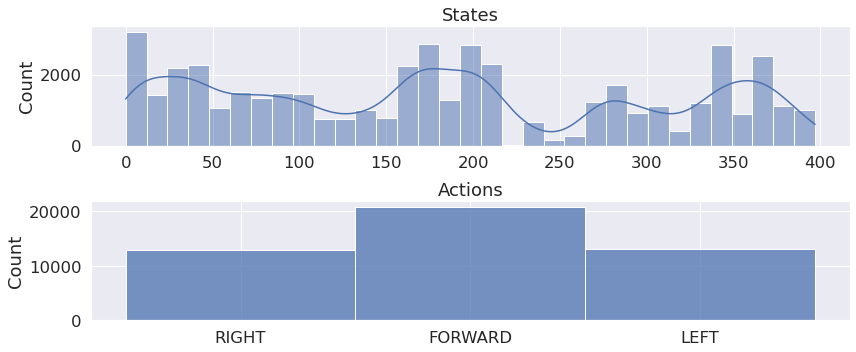
\includegraphics[height=0.4\textheight]{img/q-learning_ego_hist.png}
\end{center}
\begin{center}
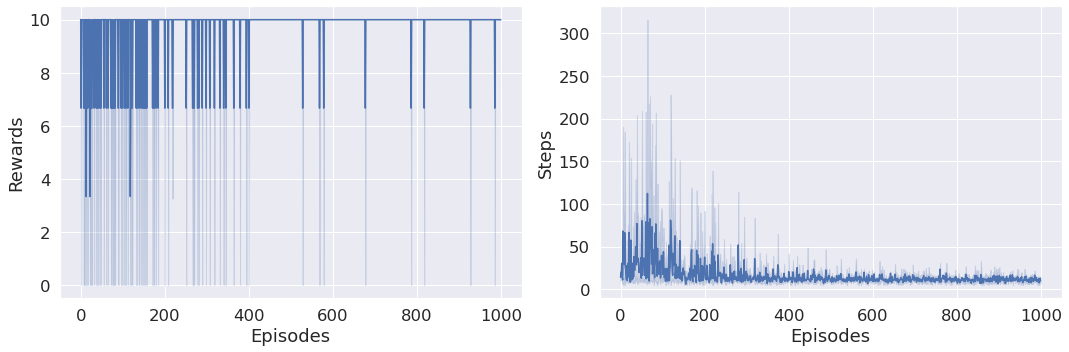
\includegraphics[height=0.4\textheight]{img/q-learning_ego_steps_rewards.png}
\end{center}
\end{frame}
\begin{frame}[label={sec:orgada6f8d}]{Standard Q-learning -- egocentric setting}
\begin{center}
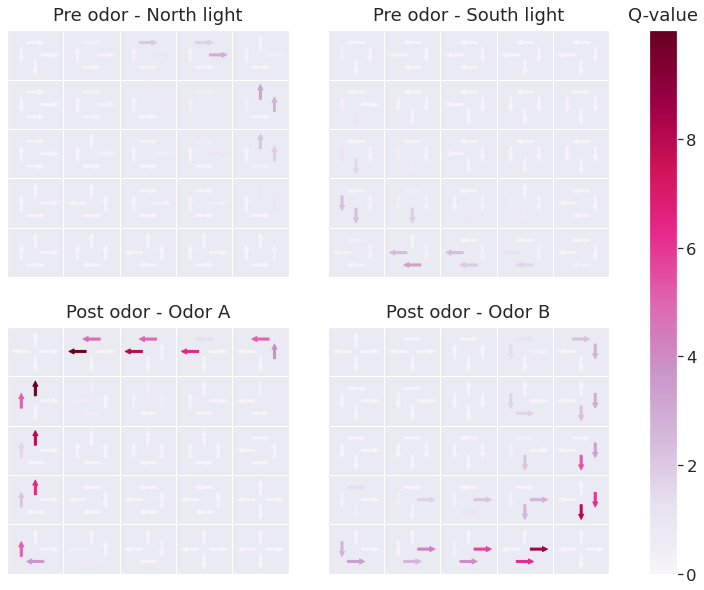
\includegraphics[height=0.9\textheight]{img/q-learning_ego_best_actions_maps.png}
\end{center}
\end{frame}
\begin{frame}[label={sec:org4b7fc0d}]{Q-learning with function approximation -- egocentric setting}
\begin{center}
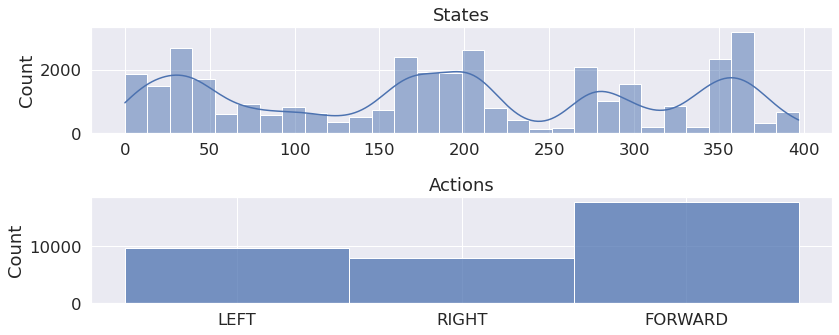
\includegraphics[height=0.4\textheight]{img/func_approx_ego_actions_states_hist_jointrep.png}
\end{center}
\begin{center}
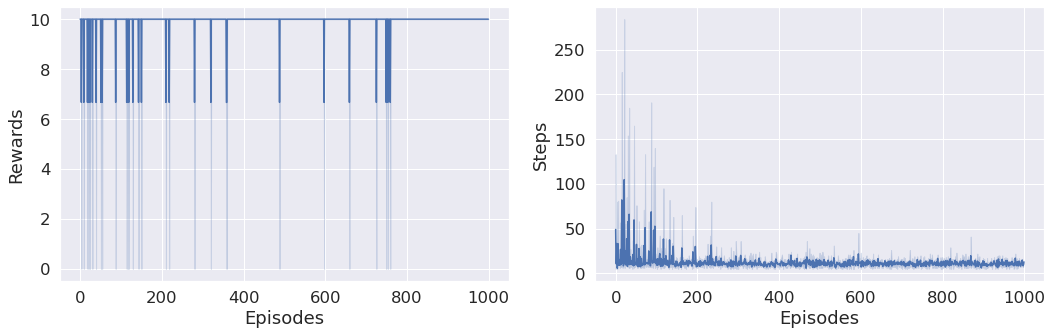
\includegraphics[height=0.4\textheight]{img/func_approx_ego_steps_rewards_jointrep.png}
\end{center}
\end{frame}
\begin{frame}[label={sec:org4c0220a}]{Q-learning with function approximation -- egocentric setting}
\begin{center}
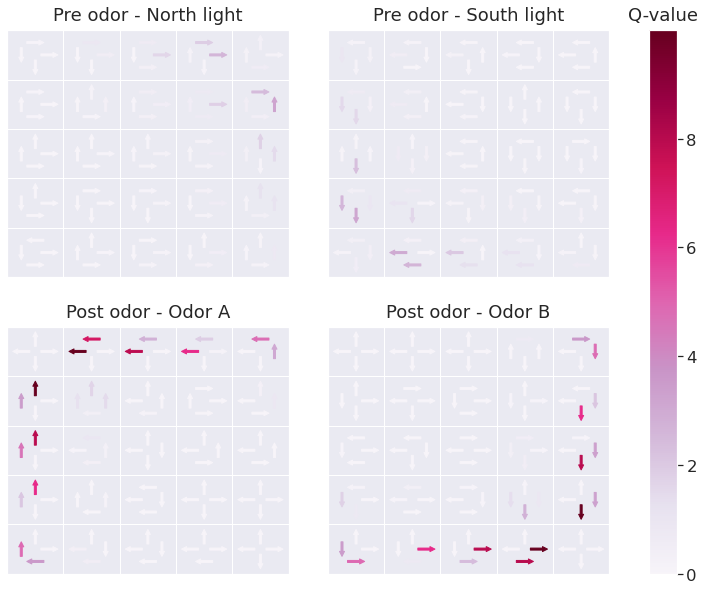
\includegraphics[height=0.85\textheight]{img/func_approx_ego_best_actions_maps_jointrep.png}
\end{center}
\end{frame}
\begin{frame}[label={sec:org95a4104}]{Location occupancy -- naive animal}
\begin{columns}
\begin{column}{0.5\columnwidth}
\begin{center}
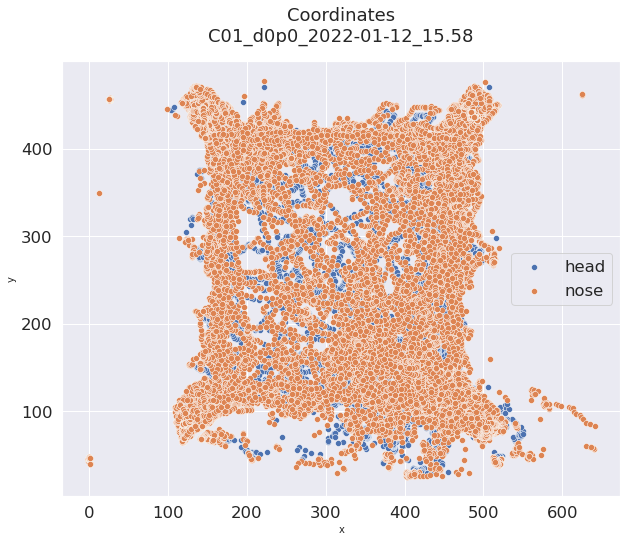
\includegraphics[width=.9\linewidth]{img/C01_d0p0_2022-01-12_15.58_coordinates.png}
\end{center}
\end{column}
\begin{column}{0.5\columnwidth}
\begin{center}
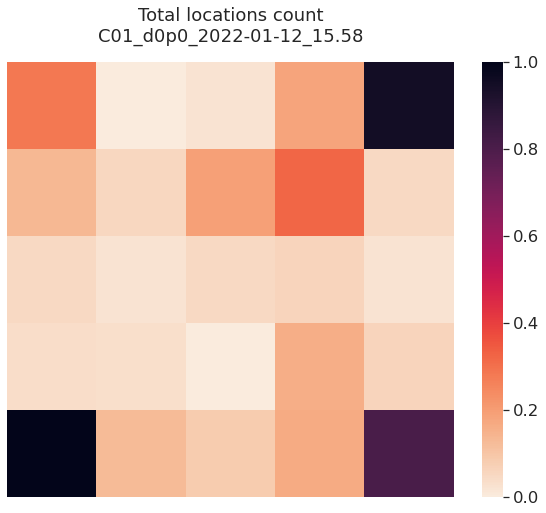
\includegraphics[width=.9\linewidth]{img/C01_d0p0_2022-01-12_15.58_locations_count.png}
\end{center}
\end{column}
\end{columns}
\begin{block}{~}
\(\to\) The locations around the ports are the most visited zones in the arena
\end{block}
\end{frame}
\begin{frame}[label={sec:orga5015db}]{Location occupancy -- animal vs. agent}
\begin{columns}
\begin{column}{0.5\columnwidth}
\begin{center}
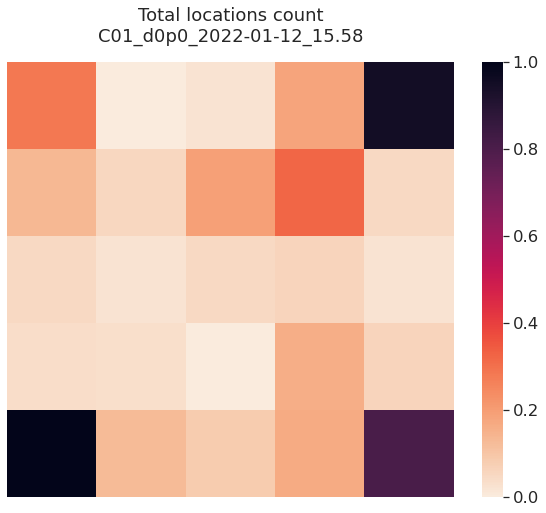
\includegraphics[height=0.43\textheight]{img/C01_d0p0_2022-01-12_15.58_locations_count.png}
\end{center}
\(\to\) The naive agent explores the space more uniformly than a real animal
\end{column}
\begin{column}{0.5\columnwidth}
\begin{center}
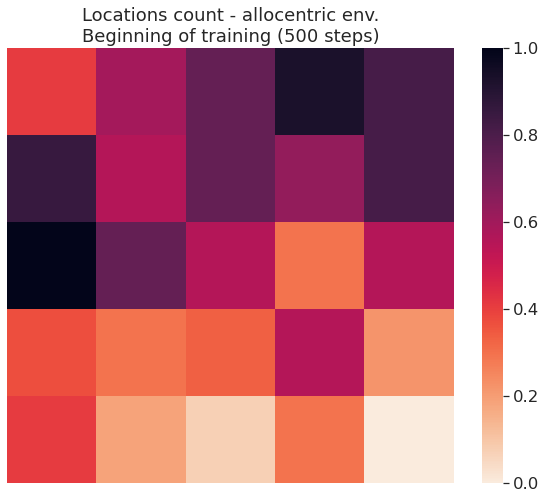
\includegraphics[height=0.4\textheight]{img/q-learning_allo_locations_count_500steps_all_cues.png}
\end{center}
\begin{center}
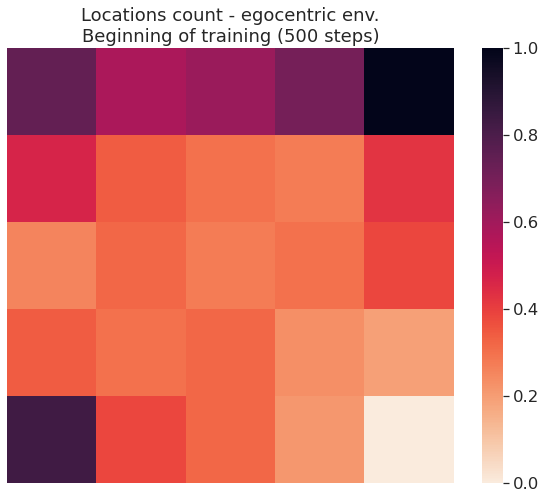
\includegraphics[height=0.4\textheight]{img/q-learning_ego_locations_count_500steps_all_cues.png}
\end{center}
\end{column}
\end{columns}
\end{frame}
\begin{frame}[label={sec:orge387630}]{Location occupancy -- allocentric vs. egocentric}
\begin{columns}
\begin{column}{0.5\columnwidth}
\footnotesize
\center
\vspace{-1em}
Allocentric
\vspace{-1em}
\begin{center}
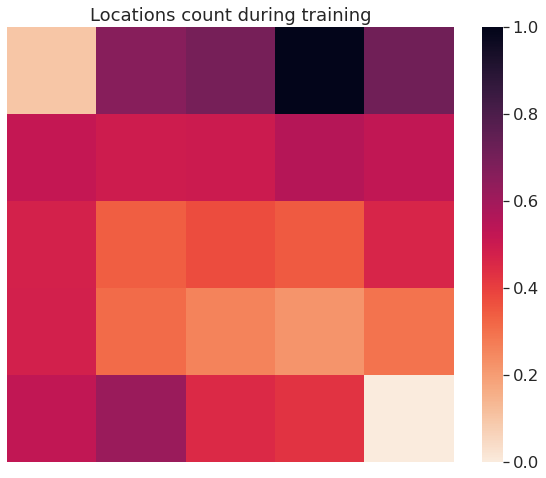
\includegraphics[height=0.2\textheight]{img/q-learning_allo_locations_count_all_steps_all_cues.png}
\end{center}

\begin{center}
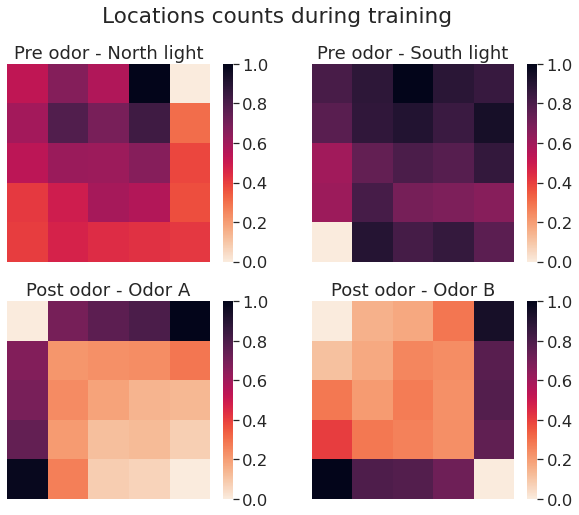
\includegraphics[width=.9\linewidth]{img/q-learning_allo_locations_count_all_steps_by_cues.png}
\end{center}
\end{column}
\begin{column}{0.5\columnwidth}
\footnotesize
\center
\vspace{-1em}
Egocentric
\vspace{-1em}
\begin{center}
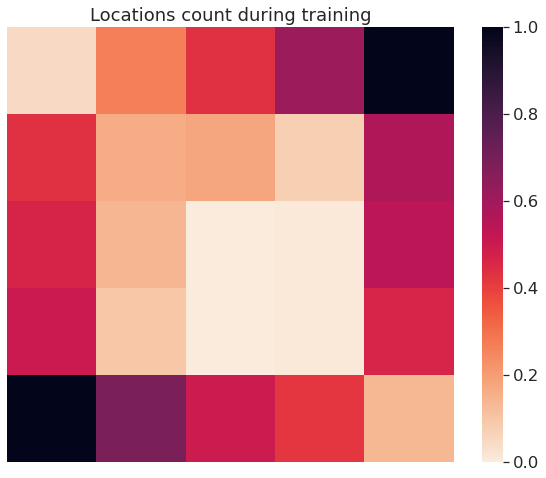
\includegraphics[height=0.2\textheight]{img/q-learning_ego_locations_count_all_steps_all_cues.png}
\end{center}

\begin{center}
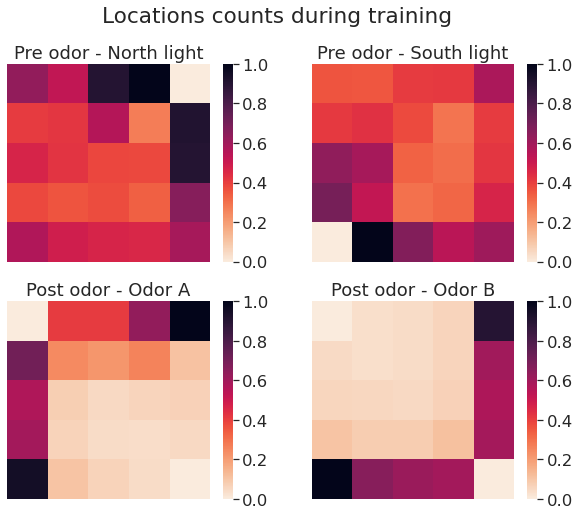
\includegraphics[width=.9\linewidth]{img/q-learning_ego_locations_count_all_steps_by_cues.png}
\end{center}
\end{column}
\end{columns}
\begin{block}{~}
\footnotesize
\vspace{-2em}
\(\to\) The egocentric agent spend more time along the walls, whereas the allocentric agent has a more homogeneous exploration of the space
\end{block}
\end{frame}
\section{Summary}
\label{sec:org818ea70}
\begin{frame}[<+->][label={sec:org506b906}]{Summary}
\begin{itemize}
\item Standard Q-learning can learn the task in \textasciitilde{}90 episodes in the \alert{allocentric} setting, and in \textasciitilde{}400 episodes in the \alert{egocentric} setting
\item Niloufar's results with function approximation in both allocentric/egocentric settings are \alert{reproducible}:
\begin{itemize}
\item The agent is \alert{not able to learn} the task \alert{without} having a place-odor joint representation
\item \alert{With} a place-odor joint representation, the agent is \alert{able to learn the task} in \textasciitilde{}60 episodes in the allocentric setting, and in \textasciitilde{}300 episodes in the egocentric setting
\end{itemize}
\end{itemize}
\end{frame}
\begin{frame}[<+->][label={sec:org77bf245}]{Summary}
\begin{itemize}
\item A naive \alert{animal} spends most of its time at the ports, whereas a naive \alert{agent} has a more uniform exploration
\item The \alert{egocentric} agent spend more time along the \alert{walls}, whereas the \alert{allocentric} agent has a more \alert{homogeneous} exploration
\end{itemize}
\end{frame}
\begin{frame}[label={sec:org709db45}]{Main differences with Niloufar's model}
\begin{columns}
\begin{column}{0.7\columnwidth}
\begin{itemize}
\item The environment is \alert{geometrically closer to the real experiment} \(\to\)~ports are in the corners of the arena, not in the middle of the walls
\item Code is clean, readable, and abstracted in high level functions/concepts
\end{itemize}
\end{column}
\begin{column}{0.3\columnwidth}
\begin{center}
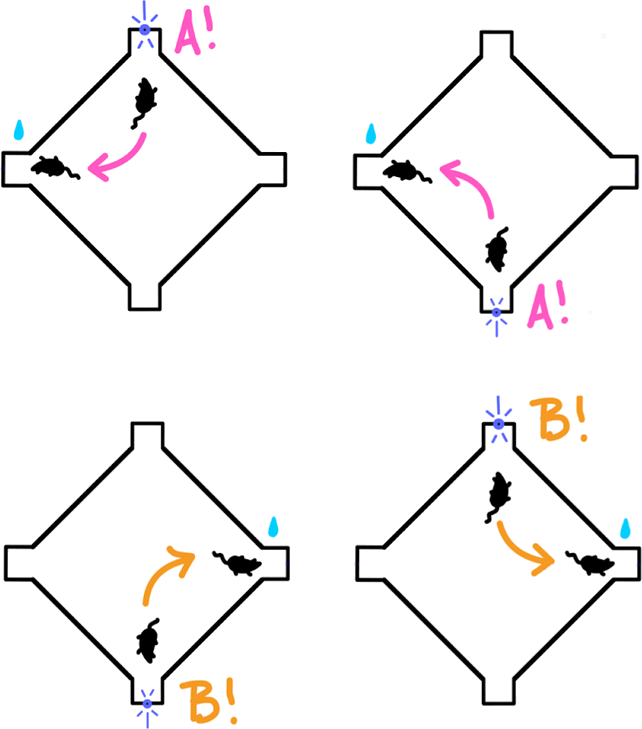
\includegraphics[width=\textwidth]{img/task.png}
\end{center}
\begin{center}
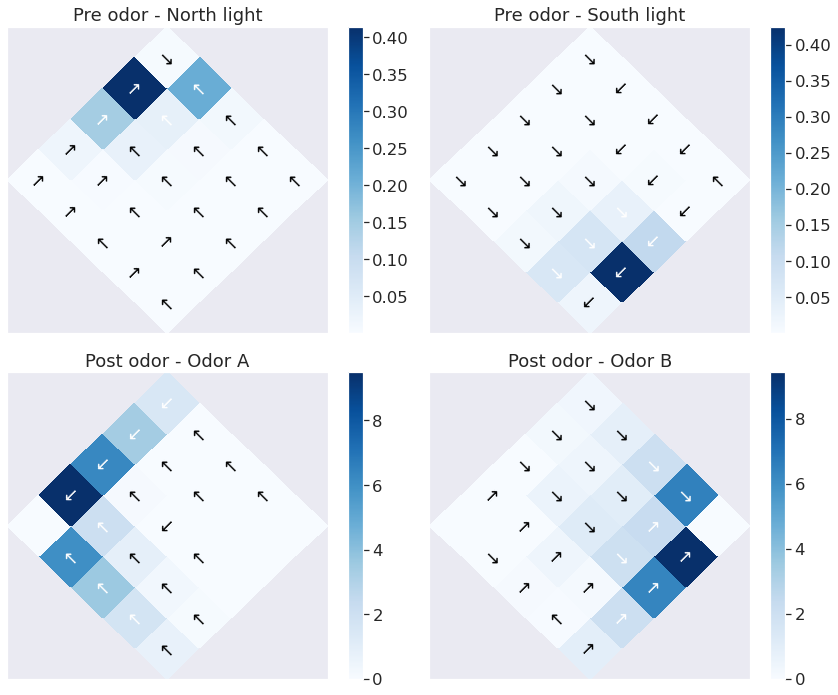
\includegraphics[width=\textwidth]{img/q-learning_allo_best_actions_maps.png}
\end{center}
\end{column}
\end{columns}
\end{frame}
\begin{frame}[<+->][label={sec:orgd3d5cfa}]{Next steps}
\begin{itemize}
\item Implement Olivia's new version of the task ?
\item Try to reduce the feature space (Jason's suggestion) \(\to\)~need to fix function approximation algorithm ?
\item Replace the manually crafted features matrix by an artificial neural network, which should learn the necessary representations to solve the task from scratch
\item \alert{NSGP seminar in \textasciitilde{}1 month}
\end{itemize}
\end{frame}
\begin{frame}[label={sec:org9b23bdc},standout]{~}
Questions ?
\end{frame}
\end{document}
